\begin{myposter}{
    Обзор литературы. Безынерционная модель.
}

    \headerbox
    {Безынерционная модель}
    {name=first,column=0,row=0,span=3}
    {
        {\huge\bf
            \begin{itemize}
                \item 2006 -- А.А. Зобова, Я.В. Татаринов -- Мобильные роботы и мехатронные системы; 2009 ПММ
                \item 2007 -- Ю.Г. Мартыненко, А.М. Формальский -- Изв. РАН. Теория сист. управл.
                \item 2011 -- А.А. Зобова -- Нелинейная динамика
                \item 2011 -- А.В. Борисов, А.А. Килин, И.С. Мамаев -- Нелинейная динамика
                \item 2014 -- А.А. Килин, А.Д. Бобыкин -- Нелинейная динамика
                \item 2018 -- Б.И. Адамов, А.И. Кобрин -- Мехатроника, автоматизация, управление
            \end{itemize}
        }
    }
    
    \headerbox
    {Обзор литературы}
    {name=second,column=0,row=1,below=first,span=3}
    {
        \vspace{10pt}
        {\huge\bf
            \begin{itemize}
                \item {
                    Экипаж состоит только из платформы и $N$ дисков колес.
                }
                \item {
                    Количество твердых тел $1 + N$.
                }
                \item {
                    Связи: для каждого колеса задан вектор $\vec{e}_i$, составляющий постоянный угол $\psi$ с плоскостью колеса, и для точек $C_i$ контакта:
                    \vspace{-15pt}
                    $$\vec{v}_{C_i} \cdot \vec{e}_i = 0$$
                }
            \end{itemize}
            \vspace{-10pt}
            \begin{figure}[H]
                \centering
                \minipage{0.45\textwidth}
                    \centering
                    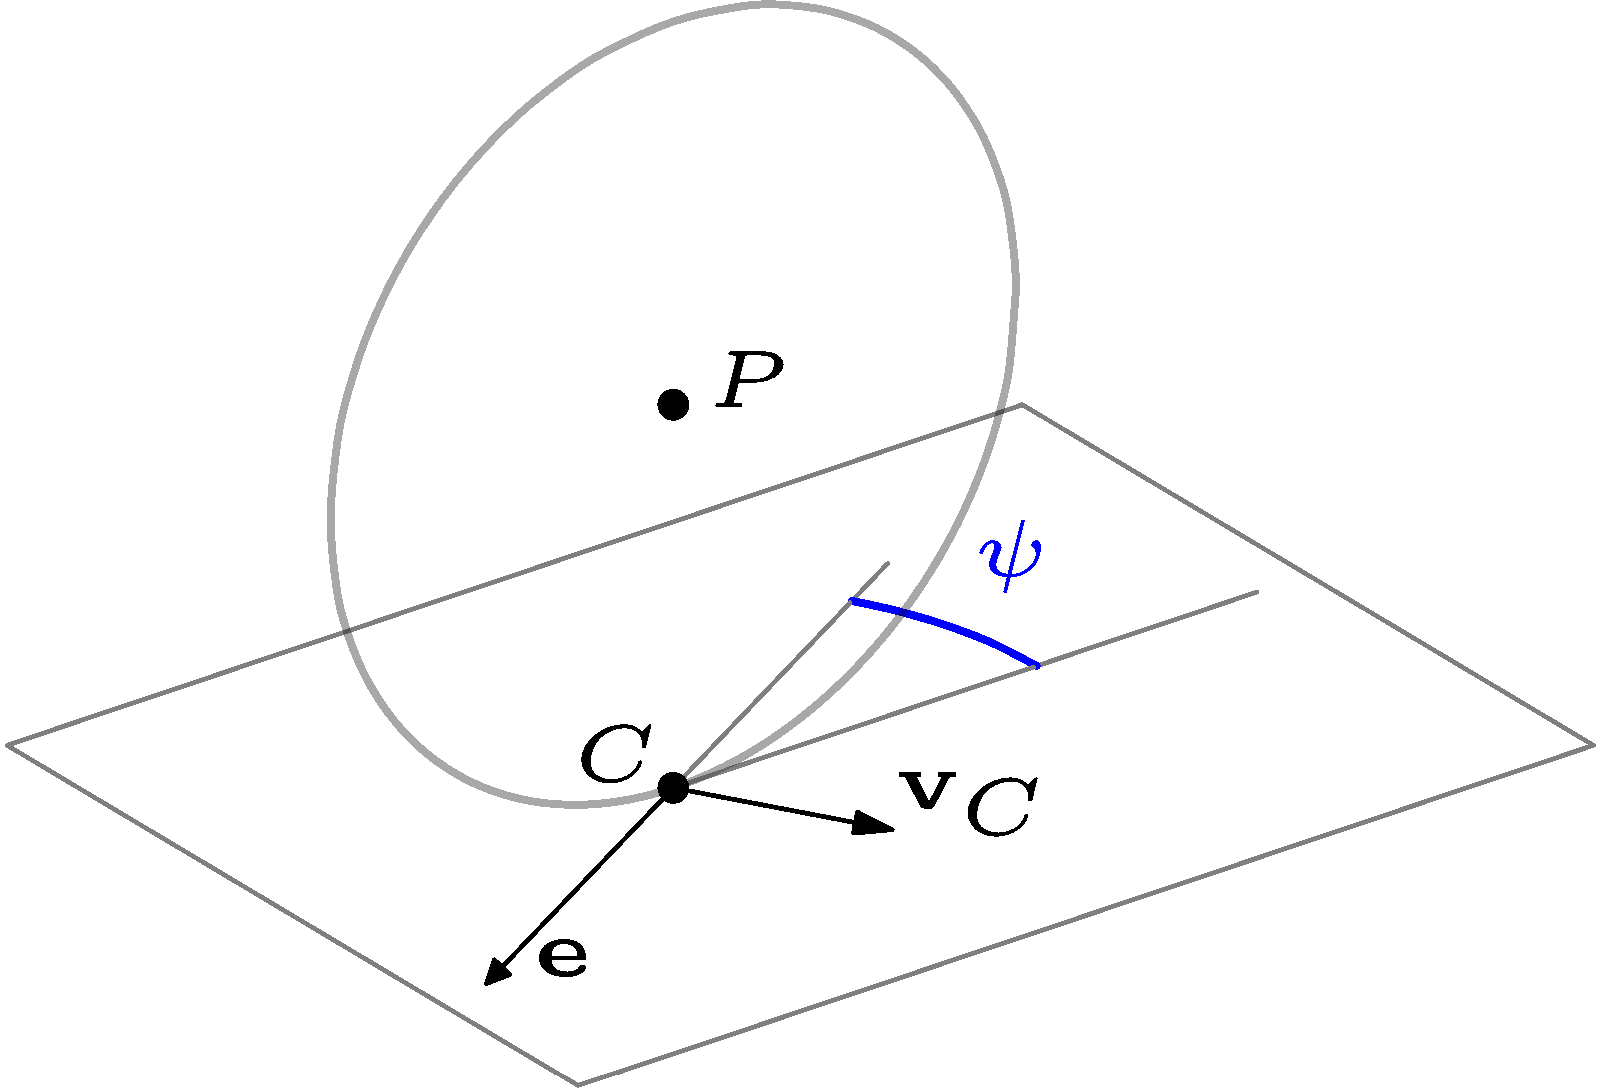
\includegraphics[width=\textwidth]{content/pic/asypng/wheel_bor.png}
                    % \asyinclude[width=\textwidth]{content/pic/asy/wheel_bor.asy}
                    \caption{Колесо}
                    \label{fig:bor_wheel_scheme}
                    % Рис.: Колесо \\
                    % .
                \endminipage
                \minipage{0.45\textwidth}
                    \centering
                    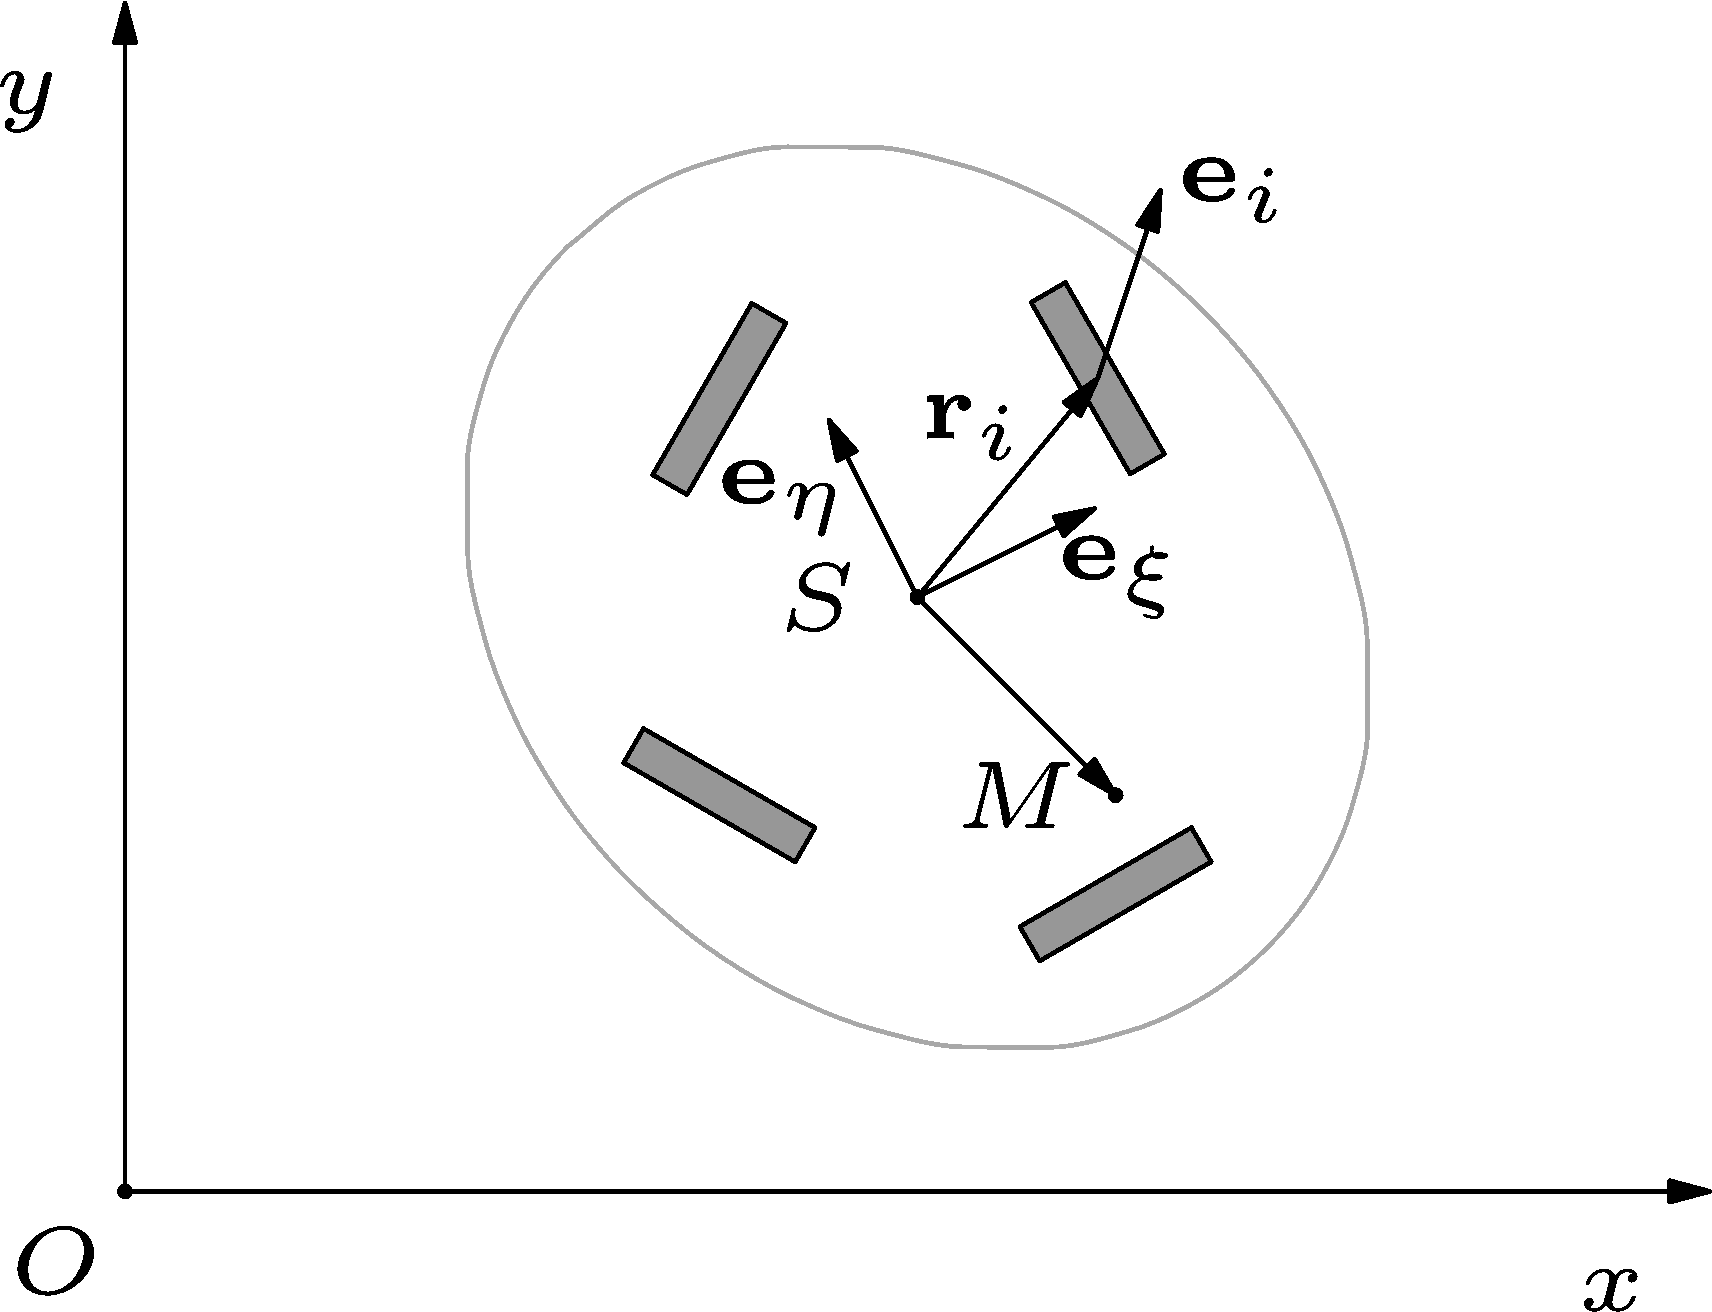
\includegraphics[width=\textwidth]{content/pic/asypng/cart_bor.png}
                    % \asyinclude[width=\textwidth]{content/pic/asy/cart_bor.asy}
                    \caption{Экипаж}
                    \label{fig:bor_vehicle}
                    % Рис.: Экипаж
                \endminipage
            \end{figure}
            \vspace{10pt}
        }
    }

\end{myposter}
